\RequirePackage{snapshot}
\documentclass[10pt,twoside]{article}

% Encoding and font setup
\usepackage[T1]{fontenc}
\usepackage[utf8]{inputenc}
\usepackage{lmodern}
\renewcommand*\familydefault{\sfdefault}

% General layout and styling
\usepackage[a4paper,left=2.5cm,right=3cm,top=2.5cm,bottom=2.5cm]{geometry}
\usepackage{graphicx,float,amssymb,amsmath}
\usepackage{natbib}
\usepackage[usenames,dvipsnames]{color}
\usepackage{tabulary}
\usepackage{fancyhdr}
\usepackage{setspace}
\usepackage[left]{lineno}
\usepackage[yyyymmdd,hhmmss]{datetime}
\usepackage{xcolor}
\usepackage{authblk}
\usepackage{subcaption}
\usepackage{titlesec}
\usepackage{nameref}
\usepackage[hidelinks]{hyperref}
\usepackage[protrusion=true,expansion=false]{microtype}
\usepackage{booktabs}
\usepackage{enumitem}

% Section and paragraph spacing customization
\titleformat{\paragraph}[hang]{\bfseries\normalsize}{\theparagraph}{1em}{}
\titlespacing*{\paragraph}{0pt}{1.5ex plus .2ex minus .2ex}{0.5em}
\newcommand{\simdataset}[1]{\vspace{1.5ex}\noindent\textbf{#1}\par\vspace{0.5ex}}

% Fancy headers/footers
\pagestyle{fancy}
\fancyhead{}
\fancyfoot{}
\fancyhead[RO,LE]{\texttt{evident}}
\fancyfoot[RO,LE]{Page-\thepage}
\fancyfoot[C]{\textbf{Preprint}}
\fancyfoot[RE,LO]{Created: \today\ at \currenttime}

% Math operators
\DeclareMathOperator{\erfc}{erfc}
\DeclareMathOperator{\erfcx}{erfcx}
\DeclareMathOperator{\erf}{erf}
\DeclareMathOperator{\erfcxinv}{erfcxinv}
\DeclareMathOperator{\Beta}{Beta}

% Margin note utilities
\newcounter{note}
\stepcounter{note}
\newcommand{\Note}[1]{\marginpar{\tiny{\color{gray}\thenote\ #1}} \stepcounter{note}}
\newcommand{\MNote}[1]{\marginpar{\tiny{\color{gray}#1}}}

\title{EVIDENT: Claim-Based Evidence Workflows for Trustworthy AI-Assisted Scientific Software}
\author[1,2]{David Teschner}
\author[1,2]{Andreas Hildebrandt}
\author[3,4,5]{Stefan Tenzer}
\author[6]{Thomas Kemmer}

\affil[1]{Institute of Computer Science, Johannes Gutenberg University, 55128 Mainz, Germany}
\affil[2]{Institute for Quantitative and Computational Biosciences (IQCB), Johannes Gutenberg University, 55128 Mainz, Germany}
\affil[3]{Helmholtz Institute for Translational Oncology, Mainz, Germany}
\affil[4]{German Cancer Research Center (DKFZ), 69120 Heidelberg, Germany}
\affil[5]{University Medical Center, Johannes Gutenberg University, 55131 Mainz, Germany}
\affil[6]{Affiliation to be added}
\date{\today}

\begin{document}

\onehalfspacing
\maketitle

\begin{abstract}
AI-assisted programming is changing how scientific software is produced. It can
reduce the effort required to generate complex code, but it also weakens a
common informal basis for trust: the assumption that the author has inspected
and understood the implementation in detail. The underlying issue is not new.
Scientific software has long relied on legacy code, copied algorithms, opaque
dependencies, numerical convention gaps, and domain-specific assumptions that
are difficult to verify. AI assistance amplifies this pre-existing trust gap by
increasing the speed and scale at which such systems can be created.

We introduce EVIDENT, a lightweight claim-based evidence workflow for
scientific software. Instead of asking whether code appears trustworthy,
EVIDENT asks what claim is being made, what evidence supports it, and what
would falsify it. Each claim is linked to a trust strategy, oracle or
reference, tolerance or decision rule, reproducible command, evidence artifact,
assumptions, and known failure modes. The framework distinguishes
implementation claims, pipeline claims, and scientific claims, and treats
understanding, validation, and proof as complementary trust strategies.

EVIDENT is not a formal standard and does not guarantee correctness. Its goal
is to make computational trust claims explicit, reviewable, and replayable. We
demonstrate the workflow using a small sealed example and a larger structural
bioinformatics case study, Proteon. Proteon shows both the strength and the
limits of claim-based evidence: many numerical claims are backed by external
oracles and tolerances, while release-grade claims also expose unresolved
pinning, replay, and artifact-preservation gaps. By treating trust as an
evidence-backed claim rather than an implicit property of code, EVIDENT
provides a practical structure for evaluating scientific software in an era
where systems can be generated faster than they can be fully inspected.
\end{abstract}

\section{Introduction}

Scientific software already has a trust gap. Computational results often
depend on legacy implementations, copied algorithms, opaque dependencies,
floating-point conventions, undocumented preprocessing steps, and tools used
beyond the user's full understanding. AI-assisted development does not create
this problem, but it changes its scale. Systems can now be produced, modified,
and optimized faster than they can be fully inspected.

The central question is therefore not whether AI-generated code is good or bad.
The question is how a scientific claim supported by software can be made
defensible when authorship and understanding are incomplete.

This paper argues that the unit of trust should not be code, but a claim about
code. A parser may claim to preserve atom coordinates. A refactor may claim to
be behavior-preserving. A GPU implementation may claim numerical equivalence to
a CPU reference. A pipeline may claim to reproduce a published figure. A
scientific analysis may claim that outputs support a domain interpretation
under stated assumptions. These claims require different evidence.

\subsection{AI-Assisted Development as an Accelerant}

Large language models for code generation and programming assistance have made
it easier to implement complex software components \citep{chen_evaluating_2021,
peng_impact_2023}. This has a real upside for scientific software. Many
projects suffer from an expertise bottleneck: the scientist may understand the
domain problem but not GPU programming, packaging, or robust interface design;
the software engineer may understand implementation but not the scientific
failure modes. AI-assisted programming can reduce the cost of crossing this
boundary by helping with boilerplate, tests, ports, interfaces, and
performance-oriented implementations that smaller groups might otherwise avoid.

The same acceleration creates a control problem. When implementation becomes
cheap, complexity can grow faster than understanding. A generated system may
compile, run, and produce plausible outputs while remaining entangled,
under-tested, or wrong in scientifically important ways. The central risk is
not that generated code can contain bugs; all code can. The risk is capability
without control: a system whose behavior matters scientifically but whose
correctness cannot be defended by the people using it. This matters whenever
low-level implementation choices are upstream of scientific evidence: parsers
can alter what observations enter an analysis, numerical kernels can change
derived quantities, preprocessing can remove or transform signals, and scoring
or filtering code can determine which results are treated as credible
downstream.

The appropriate response is not to reject AI-assisted development, but to shift
the basis of trust. Authorship alone becomes a weaker signal when code is
generated, modified, or integrated faster than it can be fully inspected.
Testing remains necessary, but unit tests mostly check whether code is
consistent with the author's expectations; they do not guarantee that those
expectations are correct. This matters especially when AI assistance helps
generate both implementation and tests. Independent oracles, reference
implementations, simulation-based ground truth, property checks, and real-world
validation corpora are how responsibility shifts from ``I wrote this'' to
``this behavior has reviewable evidence.''

AI-assisted development also raises provenance and licensing concerns that are
already familiar from scientific best practice. Scientific code is part of a
chain of intellectual provenance: known algorithms, tools, datasets, and
reference implementations should be cited, and copied or ported code should
preserve license boundaries. Generated code can obscure these relationships or
accidentally resemble licensed implementations, especially when prompted to
reproduce a known algorithm, file format, kernel, or tool behavior. Responsible
use therefore requires transparent development notes, license-aware review,
clear separation between incorporated source and clean-room reimplementation,
and documentation of the oracles and references that shaped the final system.
In scientific software, provenance, licensing, and validation are part of the
same trust argument.

\paragraph{Contributions.}
This paper makes four contributions:

\begin{enumerate}[leftmargin=*]
  \item An adaptation of claim-based assurance to everyday scientific
        software, centered on localized implementation, pipeline, and
        scientific claims.
  \item A lightweight evidence manifest linking claims to trust strategies,
        oracles, tolerances, commands, artifacts, assumptions, and failure modes.
  \item A distinction between implementation, pipeline, and scientific claims,
        preventing evidence at one layer from being silently promoted to
        another.
  \item Worked examples showing how claim-based evidence changes review,
        including a minimal claim card and a larger structural bioinformatics
        case study.
\end{enumerate}

\section{Background and Motivation}

Reproducible computational research, scientific software engineering, testing,
provenance tracking, validation against reference implementations, and formal
methods all address pieces of the trust problem
\citep{wilson2014best,sandve2013ten}. In practice, these practices are often
fragmented. A project may have unit tests, benchmark plots, release notes,
Docker files, and validation scripts, but still lack a localized answer to:
\emph{what claim is this evidence supposed to support?}

This gap matters because evidence volume is not evidence quality. A large test
suite can encode the wrong assumptions. Multiple tools can agree because they
share a convention. A benchmark can optimize for a metric that does not
correspond to the scientific claim being made. A reproducible command can
faithfully reproduce an invalid conclusion.

EVIDENT responds by making the claim explicit before evaluating the evidence.
This is a small shift in representation, but it changes review practice.
Existing practices produce tests, benchmarks, containers, reports, and
provenance records. EVIDENT localizes those artifacts around falsifiable claims
and prevents evidence from being interpreted outside the layer it actually
supports. A reviewer no longer asks only whether a project has tests or whether
a result is reproducible. The reviewer can ask whether a specific claim has an
appropriate oracle, a justified decision rule, a replay command, a preserved
artifact, and an honest statement of what the evidence does not prove.

\section{Related Work}

EVIDENT does not invent the idea that claims require evidence. It builds on
several older traditions and translates parts of them into a lightweight,
repository-level workflow for scientific software.

\paragraph{Structured argumentation and assurance cases.}
The deepest ancestry is structured argumentation. Toulmin's model describes
arguments in terms of claims, grounds, warrants, backing, qualifiers, and
rebuttals \citep{toulmin1958uses}. In engineering practice, this lineage is
most visible in safety and assurance cases, where claims about a system are
supported by structured arguments and evidence. Goal Structuring Notation (GSN)
and Claims-Arguments-Evidence (CAE) are established notations for making such
arguments explicit \citep{kelly2004goal,bloomfield2010building}. Structured
assurance case models have also been proposed for software assurance
\citep{rhodes2010software}.

EVIDENT is closest in spirit to this assurance-case literature. The difference
is target scale and use context. Assurance cases are often system-level,
regulatory, safety, or security artifacts. EVIDENT is intended to be
repo-native and close to everyday scientific software work: a parser claim, a
GPU/CPU equivalence claim, an AI-assisted refactor claim, a workflow replay
claim, or a scientific interpretation claim.

\paragraph{Verification and validation in scientific computing.}
Scientific computing has long treated trust as evidence-relative and
context-dependent. Verification, validation, and uncertainty quantification
provide frameworks for assessing credibility in modeling and simulation,
including code verification, solution verification, model validation, predictive
capability, and uncertainty propagation
\citep{oberkampf2002verification,roy2011comprehensive}. EVIDENT is less
ambitious and less domain-specific than full V\&V/UQ practice. It does not
estimate predictive uncertainty or replace model validation. Instead, it
borrows the discipline of explicit context, decision rules, and limits, and
applies it to a broader set of scientific-software claims.

\paragraph{Reproducibility, provenance, and artifact review.}
Reproducible research and research-software engineering provide practical
guidance for version control, dependency capture, automation, testing,
documentation, and reusable artifacts
\citep{sandve2013ten,wilson2014best}. Artifact review and badging systems
further encourage authors to provide artifacts that can be inspected, reused,
or used to validate results \citep{acm_artifact_badging}. Provenance models
and software citation principles address traceability, credit, and persistent
identification of the software and data involved in computation
\citep{w3c_prov_dm,smith2016software,barker2022fair}. These practices are
necessary but not sufficient for claim review. Provenance records how an
artifact was produced; EVIDENT records what claim that artifact is evidence
for.

\paragraph{AI-assisted software development.}
Large language models trained on code have made software generation and
modification substantially easier \citep{chen_evaluating_2021}. Empirical work
on tools such as GitHub Copilot reports productivity gains
\citep{peng_impact_2023}, while test-driven and interactive workflows explore
ways to clarify intent and improve generated-code correctness
\citep{fakhoury2024ticoder}. EVIDENT treats AI assistance as an accelerant,
not the root cause of the trust problem. Its role in this paper is to motivate
why authorship and informal inspection become weaker proxies for trust, and why
external oracles, replayable artifacts, and explicit failure modes become more
important.

\section{Claim-Based Evidence}

An EVIDENT claim links a statement about software behavior to the evidence used
to justify it:

\begin{center}
\small\ttfamily
\begin{tabular}{l}
claim -> trust strategy -> oracle/reference \\
-> tolerance or decision rule -> reproducible command \\
-> artifact -> assumptions and failure modes
\end{tabular}
\end{center}

The workflow uses three complementary trust strategies:

\begin{itemize}[leftmargin=*]
  \item \textbf{Understanding}: explaining why the component should work.
  \item \textbf{Validation}: showing that the component behaves correctly
        against an oracle, reference, property, or benchmark.
  \item \textbf{Proof}: guaranteeing properties under defined assumptions.
\end{itemize}

Most practical scientific software combines these strategies. The less we
understand a component by inspection, the stronger the validation must be.

\begin{figure}[t]
  \centering
  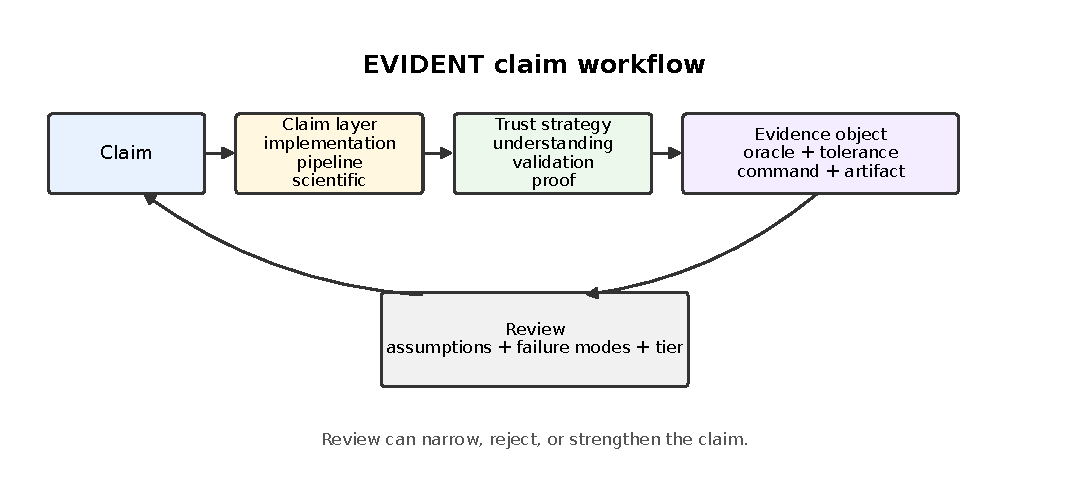
\includegraphics[width=0.95\linewidth]{figures/evident_workflow.pdf}
  \caption{EVIDENT organizes trust around localized claims. Each claim is
  placed in a layer, assigned one or more trust strategies, connected to an
  evidence object, and reviewed through assumptions, failure modes, and tier.
  Failed evidence can narrow, reject, or strengthen the claim.}
  \label{fig:evident-workflow}
\end{figure}

\subsection{What Counts as a Claim?}

In EVIDENT, a claim is not a slogan about a project. It is a localized statement
that can be reviewed. Examples include:

\begin{itemize}[leftmargin=*]
  \item a parser preserves atom coordinates and hierarchy for a defined class
        of PDB/mmCIF files;
  \item a CUDA kernel is numerically equivalent to a CPU reference within a
        stated tolerance;
  \item an AI-assisted refactor preserves the behavior of a previous
        implementation on a representative corpus;
  \item a pipeline reproduces a table or figure from a previous release;
  \item a workflow's outputs support a scientific interpretation under stated
        assumptions.
\end{itemize}

This localization is important because different claims require different
evidence. A unit test can support an implementation claim. It rarely supports a
scientific claim by itself. A benchmark can support a performance claim. It
does not automatically support a correctness claim. A simulation with known
ground truth can strongly validate modeled behavior, but its authority ends
where the simulator's assumptions end.

\subsection{Claim Layers}

EVIDENT distinguishes three claim layers:

\begin{description}
  \item[Implementation claim] A component behaves according to a specification.
  \item[Pipeline claim] A workflow transforms inputs into outputs reproducibly.
  \item[Scientific claim] Outputs support an interpretation under stated
        assumptions.
\end{description}

Evidence for one layer does not automatically validate the next. For example,
showing that a parser preserves coordinates does not prove that a downstream
biological interpretation is valid. Showing that a workflow reproduces a figure
does not prove that the figure supports the manuscript's conclusion.

\begin{figure}[t]
  \centering
  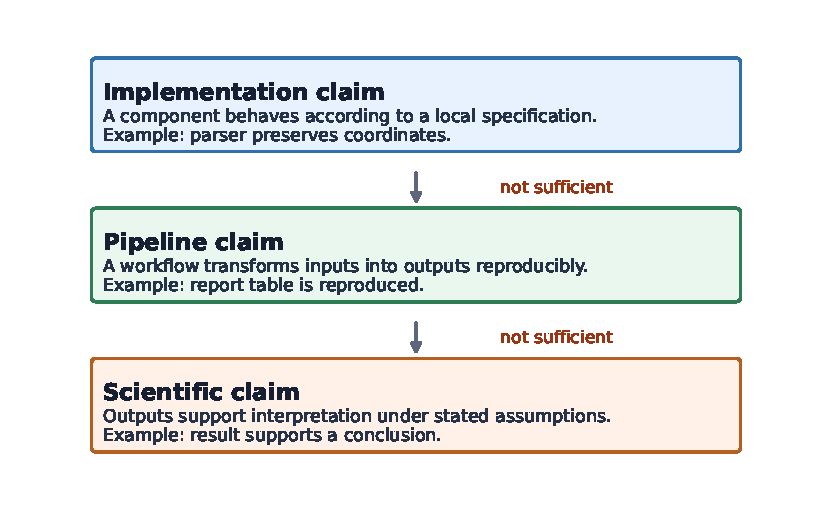
\includegraphics[width=0.90\linewidth]{figures/claim_layers.pdf}
  \caption{Evidence should not be silently promoted across claim layers.
  Implementation evidence, pipeline validity, and scientific interpretation are
  related, but each requires its own assumptions and decision rules.}
  \label{fig:claim-layers}
\end{figure}

\section{The EVIDENT Workflow}

EVIDENT provides a manifest schema and lightweight validation tooling
\citep{evident_repo}. A claim contains a stable identifier, a claim kind, a
tier, a subsystem, inputs, outputs, pinned versions, tolerances, evidence
commands, artifacts, assumptions, and failure modes. The schema is deliberately
machine-queryable: claims can be filtered by subsystem, oracle, tier,
capability, or tolerance.

\begin{table}[h]
\centering
\caption{Core EVIDENT manifest fields.}
\begin{tabular}{ll}
\toprule
Field & Role \\
\midrule
\texttt{id} & Stable claim identifier \\
\texttt{claim} & Human-readable statement being justified \\
\texttt{trust\_strategy} & Understanding, validation, proof, or combination \\
\texttt{oracle} & External tool, reference implementation, or benchmark \\
\texttt{tolerances} & Decision rule for accepting or rejecting evidence \\
\texttt{command} & Replay command \\
\texttt{artifact} & Persisted evidence output \\
\texttt{assumptions} & Conditions under which the claim is interpreted \\
\texttt{failure\_modes} & Known ways the evidence can mislead \\
\bottomrule
\end{tabular}
\end{table}

\subsection{Claim Tiers}

Claims are assigned a tier. The tier is not a prestige label; it states how the
evidence is used.

\begin{description}
  \item[CI-tier] Evidence is cheap enough to run during routine development.
        These claims guard regressions but are usually limited in input scale
        or oracle coverage.
  \item[Release-tier] Evidence is intended to justify a public release. These
        claims should pin the project version, oracle versions, input corpus,
        replay command, and artifact.
  \item[Research-tier] Evidence is informative but not yet release-gating. This
        tier is useful for emerging components, exploratory benchmarks, or
        claims whose oracles are still incomplete.
\end{description}

Separating tiers prevents a common failure mode: treating a fast smoke test as
if it were release-grade validation, or treating exploratory evidence as if it
were a stable public contract.

\subsection{Review Questions}

The manifest is designed to make review mechanical before it becomes
philosophical. A reviewer can ask:

\begin{itemize}[leftmargin=*]
  \item Is the claim specific enough to falsify?
  \item Does the oracle or reference actually bear on the claim?
  \item Is the tolerance stated before interpretation of the result?
  \item Is the replay command executable in a documented environment?
  \item Is the artifact preserved, or is the evidence only described?
  \item Are assumptions and convention gaps visible?
  \item Is an implementation claim being over-promoted into a scientific claim?
\end{itemize}

These questions are deliberately modest. They do not decide scientific truth.
They make clear what is being asserted and what evidence is being offered.

\section{Case Study 1: A Minimal Claim Card}

The first example is intentionally small. Its purpose is to show closure rather
than domain complexity. Consider an implementation of Welford's online
algorithm for mean and variance. The scientific content is minimal, but the
evidence structure is complete.

\begin{table}[h]
\centering
\caption{Example of a minimal EVIDENT claim card.}
\begin{tabular}{p{0.22\linewidth}p{0.68\linewidth}}
\toprule
Field & Example content \\
\midrule
Claim & The Welford implementation computes mean and sample variance equivalent
to NumPy on a fixed edge-case corpus. \\
Trust strategy & Validation, supported by understanding of the recurrence. \\
Oracle & NumPy \texttt{mean} and \texttt{var(ddof=1)}. \\
Inputs & Empty arrays, singletons, constant arrays, large-offset arrays,
alternating signs, and pseudorandom vectors with fixed seed. \\
Tolerance & Absolute error $<10^{-12}$ for small values; relative error
$<10^{-10}$ for large values; documented behavior for empty inputs and NaNs. \\
Command & \texttt{python validation/welford\_oracle.py}. \\
Artifact & \texttt{validation/artifacts/welford\_oracle.json}. \\
Assumptions & NumPy is treated as the reference for the tested floating-point
semantics; platform-level differences are not expected to dominate. \\
Failure modes & Does not prove numerical stability for arbitrary streaming
orders; does not cover non-IEEE arithmetic or distributed reductions. \\
\bottomrule
\end{tabular}
\end{table}

The important feature is not that this is a difficult validation problem. It is
that every part of the trust argument has a place. The claim is falsifiable; the
oracle is named; the tolerance is explicit; the command can be replayed; the
artifact can be inspected; the assumptions and gaps are visible.

This example also illustrates the difference between understanding and
validation. A reviewer may understand Welford's recurrence and still want
validation against edge cases where naive implementations fail, such as
large-offset data where catastrophic cancellation affects one-pass formulas.
Understanding explains why the algorithm should work; validation checks that
this implementation actually behaves as claimed.

The same claim can be represented directly in a manifest:

\begin{verbatim}
id: welford.mean_variance.numpy_equivalence
kind: measurement
trust_strategy: [understanding, validation]
claim: >
  The Welford implementation computes mean and sample variance
  equivalent to NumPy on a fixed edge-case corpus.
evidence:
  oracle: [NumPy]
  command: python validation/welford_oracle.py
  artifact: validation/artifacts/welford_oracle.json
tolerances:
  - metric: absolute_error
    op: "<"
    value: 1.0e-12
    prose: small-value mean and variance agreement
assumptions:
  - NumPy is treated as the floating-point reference.
failure_modes:
  - Does not cover arbitrary distributed reduction order.
\end{verbatim}

\section{Case Study 2: Mapping Claim Coverage in a Realistic Toolkit}

Proteon is a Rust-first structural bioinformatics toolkit with Python and CLI
entry points \citep{proteon_repo}. It implements components where plausible
output is insufficient: structure I/O, alignment, solvent-accessible surface
area, secondary structure assignment, hydrogen placement, force-field energies,
minimization, search, and dataset export.

Proteon is a useful EVIDENT case because its claims vary in maturity. Some are
CI-tier claims over small fixtures. Some are release-tier claims over larger
corpora. Some are research-tier claims where the evidence is useful but not yet
release-gating. This creates a realistic trust envelope rather than a polished
toy.

\begin{table}[h]
\centering
\caption{Examples of Proteon claims expressed in EVIDENT form.}
\small
\begin{tabular}{p{0.22\linewidth}p{0.13\linewidth}p{0.18\linewidth}p{0.36\linewidth}}
\toprule
Claim area & Tier & Oracle/reference & Evidence purpose \\
\midrule
PDB/mmCIF I/O & CI & Biopython, Gemmi & Check counts, coordinates,
hierarchy, metadata, and edge-case parsing behavior. \\
TM-align & CI & USAlign & Bound TM-score, RMSD, and aligned-length drift
against a C++ reference implementation. \\
SASA & CI/release & Biopython & Check pointwise fixture behavior and
distributional behavior on a larger corpus. \\
DSSP & CI & pydssp & Check secondary-structure assignments after
collapsing to a shared three-class alphabet. \\
Hydrogen placement & CI & reduce & Check rigid hydrogen placement within a
geometric tolerance. \\
AMBER96/OBC energy & Release & OpenMM & Check energy components or totals
under explicitly matched nonbonded and solvent conventions. \\
MSA/search features & Research & MMseqs2 & Compare shared-hit residue and
deletion agreement while documenting known boundary convention gaps. \\
\bottomrule
\end{tabular}
\end{table}

\subsection{Oracle-Backed Claims}

Proteon's evidence model relies primarily on validation against independent
tools:

\begin{itemize}[leftmargin=*]
  \item structure I/O against Biopython and Gemmi;
  \item TM-align behavior against USAlign and related C++ references
        \citep{zhang2005tmalign};
  \item SASA against Biopython and planned FreeSASA coverage;
  \item DSSP-style secondary structure against pydssp;
  \item hydrogen placement against reduce;
  \item AMBER96 and OBC energy components against OpenMM;
  \item sequence/search-related behavior against MMseqs2-style oracles
        \citep{soeding2005protein}.
\end{itemize}

Each claim should state the oracle, tolerance, command, artifact, assumptions,
and failure modes. The important point is not that any one oracle proves
correctness. The important point is that each claim says what the oracle can and
cannot justify.

\subsection{Tolerance as Part of the Claim}

Proteon illustrates why tolerances must be first-class evidence, not informal
test constants. Floating-point implementations can differ because of operation
ordering, compiler flags, GPU execution, or legitimate convention choices. In
structural bioinformatics, tools may also differ in atom filtering, chain
ordering, hydrogen placement policy, nonbonded cutoffs, or secondary-structure
alphabet. A tolerance therefore encodes a scientific and computational
judgment.

For example, a tight tolerance is appropriate when comparing deterministic
energy components under matched force-field and cutoff settings. A wider or
asymmetric tolerance may be appropriate where two tools follow related but not
identical conventions. In such cases, EVIDENT requires the convention gap to be
documented rather than hidden behind a passing test.

\subsection{Fast CI and Heavy Release Evidence}

Proteon also shows a common practical split. Some oracles are cheap enough to
run continuously. Others, such as large OpenMM, GROMACS, or corpus-scale
retrieval runs, are expensive to install or execute. EVIDENT does not require
all evidence to run on every commit. It requires that the role of each evidence
source be explicit. A CI-tier test can prevent routine regressions, while a
release-tier claim can require a heavier replay before tagging.

This distinction is especially important for AI-assisted development. Generated
or heavily refactored code may be easy to produce but expensive to validate
fully. Claim tiers allow development to remain fast without pretending that
fast evidence is complete evidence.

\subsection{Failed Claims and Claim Narrowing}

An evidence workflow should not only store passing results. Failed claims are
scientifically useful because they show where a claim was too broad, an oracle
was inappropriate, or a tolerance encoded the wrong assumption. In EVIDENT, a
failed replay should lead to one of three outcomes: the implementation is fixed,
the claim is rejected, or the claim is narrowed until it matches the evidence.
For example, a broad claim that an alignment implementation ``matches the
reference'' may become a narrower claim about TM-score agreement under a
particular normalization, fixture set, and tolerance. This narrowing is not a
failure of the framework. It is the framework doing useful work: preventing
evidence from supporting more than it can justify.

\subsection{What EVIDENT Reveals}

The Proteon case also shows why explicit claims are useful. The manifest makes
trust gaps visible:

\begin{itemize}[leftmargin=*]
  \item some release corpora still need content-addressed hashes;
  \item some artifacts live outside the repository and need preservation;
  \item some oracle versions are placeholders awaiting release pinning;
  \item some tests skip when heavy oracles are not installed;
  \item some evidence is internal reference shadowing rather than independent
        validation;
  \item search is explicitly research-tier rather than release-grade.
\end{itemize}

These are not failures of the approach. They are precisely the kind of review
information that an evidence workflow should expose.

\subsection{Review Outcome}

The Proteon case does not support the conclusion ``Proteon is correct.'' That
would be too broad. It supports a more useful conclusion: different Proteon
claims have different evidence status. Some implementation claims are guarded
by CI oracles. Some release claims are supported by larger validation runs but
still need stronger corpus and artifact pinning. Some research claims are
clearly marked as exploratory. The framework turns a vague trust discussion
into a reviewable map of claim coverage.

\section{Discussion}

EVIDENT should be understood as a review instrument, not a correctness proof.
It helps reviewers ask sharper questions:

\begin{itemize}[leftmargin=*]
  \item Is the claim clear?
  \item Is the oracle meaningful?
  \item Is the tolerance justified?
  \item Is the replay command executable?
  \item Is the artifact preserved?
  \item Are assumptions and failure modes explicit?
  \item Is evidence at one layer being over-promoted to another?
\end{itemize}

The framework is intentionally modest. It does not replace domain expertise,
formal verification, code review, or statistical validation. It gives those
activities a common object: a reviewable claim with evidence.

\subsection{Relation to Existing Practice}

Many scientific software projects already contain the ingredients used by
EVIDENT:
unit tests, benchmark scripts, Docker files, oracle comparisons, frozen
fixtures, validation reports, and release notes. EVIDENT does not claim that
these practices are new. Its contribution is organizational. It binds evidence
to claims and makes the limits of each source explicit.

A skeptical reader might therefore ask whether EVIDENT is simply testing,
provenance, and reproducibility with a YAML file. The answer is no. EVIDENT
does not invent testing, provenance, or reproducibility. It binds them to
localized, falsifiable claims and prevents evidence from being interpreted
outside its scope. The manifest is not the contribution by itself; the
claim-centered review discipline is.

This binding matters during review. Without it, a project can accumulate
artifacts without knowing what they prove. With it, gaps become visible: a
claim without an oracle is incomplete, a benchmark without a decision rule is
descriptive but not validating, a replay command without a preserved artifact
is weaker than it looks, and a tolerance without rationale is an implicit
scientific judgment.

\subsection{AI Assistance Changes the Burden, Not the Standard}

The standard for accepting scientific results should not be relaxed because code
is easier to produce. If anything, the validation burden becomes more explicit.
AI assistance can make implementation cheaper, but correctness, provenance, and
scientific interpretation remain expensive. EVIDENT provides a place to account
for that cost. It asks authors to say what was claimed, how it was checked, what
would falsify it, and where the evidence stops.

This also changes the role of code review. In AI-assisted scientific
programming, line-by-line inspection alone becomes an increasingly poor proxy
for trust: reviewers cannot reasonably inspect every generated implementation in
detail. They can, however, inspect the claims being made, the oracles used, the
decision rules applied, and the artifacts preserved. This is the practical
review shift EVIDENT is designed to support.

\section{Limitations}

EVIDENT can make weak evidence visible, but it cannot make it strong. It can
record an oracle, but it cannot guarantee that the oracle is correct. It can
require a tolerance, but it cannot decide whether that tolerance is
scientifically meaningful. It can preserve artifacts, but it cannot ensure that
a reviewer interprets them well.

The workflow also introduces maintenance burden. Claims must be updated when
oracles drift, corpora change, or commands stop replaying. A stale claim is
dangerous because it has the appearance of structure without current evidence.
Future work should therefore include automated replay status, stale-evidence
warnings, and requirement-profile queries.

The current framework is intentionally lightweight. It does not yet define
a universal ontology for scientific claims, and it should probably avoid doing
so prematurely. Different domains need different oracles, tolerances, and
failure modes. A useful framework must be strict enough to support review but
flexible enough to admit domain-specific evidence.

\section{Conclusion}

AI-assisted programming exposes and amplifies a pre-existing weakness in
scientific software: trust is often implicit, informal, and poorly localized.
EVIDENT proposes a lightweight response. It turns ``trust me'' into a
reviewable claim with evidence.

The central shift is simple: the unit of trust is not code, but a claim about
code. When claims are explicit, evidence can be judged, replayed, challenged,
and improved.

\bibliographystyle{plainnat}
\bibliography{references}

\end{document}
